\chapter{Bi-directional RNN (BRNN/ BiRNN) (1997)}


\begin{figure}[H]
    \centering
    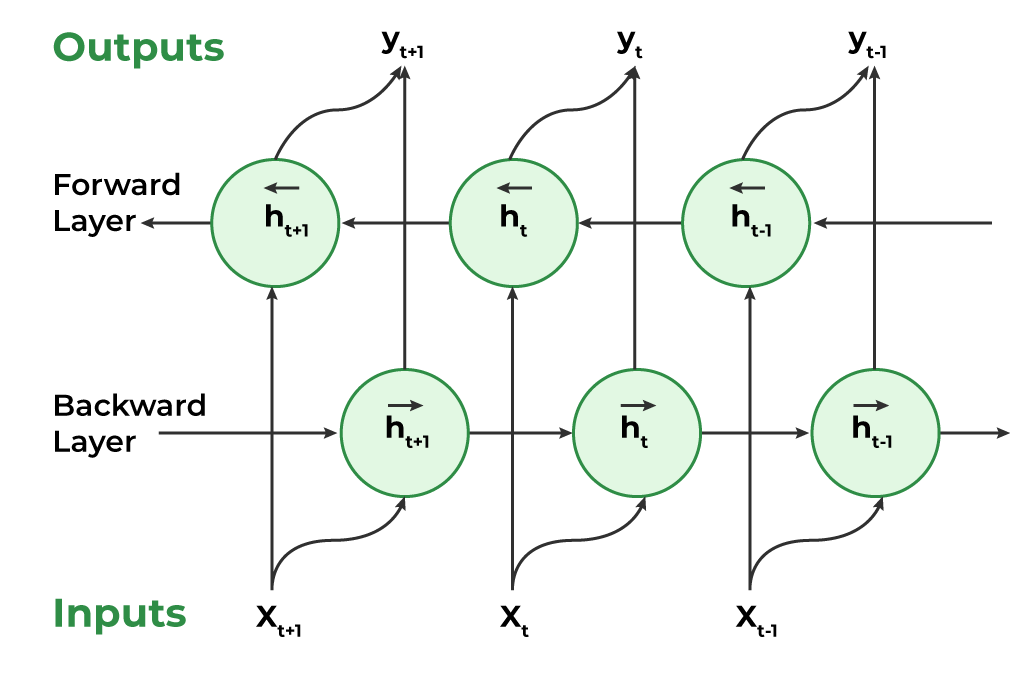
\includegraphics[
        width=\linewidth,
        height=5cm,
        keepaspectratio,
    ]{images/recurrent-neural-networks/birnn-gfg.fig-1.png}
\end{figure}

\begin{enumerate}
    \item A Bidirectional Recurrent Neural Network (BRNN) is an extension of the traditional RNN that processes sequential data in both forward and backward directions. 
    This allows the network to utilize both past and future context when making predictions providing a more comprehensive understanding of the sequence.
    \hfill \cite{geeksforgeeks/deep-learning/bidirectional-recurrent-neural-network}
\end{enumerate}



\section{Working of Bidirectional Recurrent Neural Networks}

\begin{enumerate}
    \item \textbf{Inputting a Sequence}: A sequence of data points each represented as a vector with the same dimensionality is fed into the BRNN. 
    The sequence may have varying lengths.
    \hfill \cite{geeksforgeeks/deep-learning/bidirectional-recurrent-neural-network}

    \item \textbf{Dual Processing}: BRNNs process data in two directions:
    \hfill \cite{geeksforgeeks/deep-learning/bidirectional-recurrent-neural-network}
    \begin{enumerate}
        \item \textbf{Forward direction}: The hidden state at each time step is determined by the current input and the previous hidden state.
        \hfill \cite{geeksforgeeks/deep-learning/bidirectional-recurrent-neural-network}
    
        \item \textbf{Backward direction}: The hidden state at each time step is influenced by the current input and the next hidden state.
        \hfill \cite{geeksforgeeks/deep-learning/bidirectional-recurrent-neural-network}
    \end{enumerate}

    \item \textbf{Computing the Hidden State}: A non-linear activation function is applied to the weighted sum of the input and the previous hidden state creating a memory mechanism that allows the network to retain information from earlier steps.
    \hfill \cite{geeksforgeeks/deep-learning/bidirectional-recurrent-neural-network}

    \item \textbf{Determining the Output}: A non-linear activation function is applied to the weighted sum of the hidden state and output weights to compute the output at each step. 
    This output can either be:
    \hfill \cite{geeksforgeeks/deep-learning/bidirectional-recurrent-neural-network}
    \begin{enumerate}
        \item The final output of the network.
        \hfill \cite{geeksforgeeks/deep-learning/bidirectional-recurrent-neural-network}
    
        \item An input to another layer for further processing.
        \hfill \cite{geeksforgeeks/deep-learning/bidirectional-recurrent-neural-network}
    \end{enumerate}
\end{enumerate}




\begin{lstlisting}[
    language=Python,
    caption=BiRNN from scratch (PyTorch) \cite{common/online/chatgpt}
]
class BidirectionalVanillaRNN(nn.Module):
    def __init__(self, input_size, hidden_size, output_size):
        """
        hidden_size: size per direction. 
            final concatenated hidden will be hidden_size * 2
        """
        super().__init__()
        self.input_size = input_size
        self.hidden_size = hidden_size
        # FORWARD direction params
        self.Wx_f = nn.Parameter(torch.randn(input_size, hidden_size) * 0.1)
        self.Wh_f = nn.Parameter(torch.randn(hidden_size, hidden_size) * 0.1)
        self.bh_f = nn.Parameter(torch.zeros(hidden_size))
        # BACKWARD direction params
        self.Wx_b = nn.Parameter(torch.randn(input_size, hidden_size) * 0.1)
        self.Wh_b = nn.Parameter(torch.randn(hidden_size, hidden_size) * 0.1)
        self.bh_b = nn.Parameter(torch.zeros(hidden_size))

        # final classifier from concatenated hidden (h_f_last || h_b_last)
        self.Why = nn.Parameter(torch.randn(hidden_size * 2, output_size) * 0.1)
        self.by = nn.Parameter(torch.zeros(output_size))

    def forward(self, x, h0_f=None, h0_b=None):
        """
        x: (batch, seq_len, input_size)
        returns logits (batch, output_size), 
            and tuple of last forward/backward hidden states
        """
        batch, seq_len, _ = x.shape
        # init hidden states
        if h0_f is None:
            h_f = x.new_zeros(batch, self.hidden_size)
        else:
            h_f = h0_f
        if h0_b is None:
            h_b = x.new_zeros(batch, self.hidden_size)
        else:
            h_b = h0_b

        # forward pass (t = 0 .. seq_len-1)
        for t in range(seq_len):
            xt = x[:, t, :]                       # (batch, input_size)
            pre_f = xt @ self.Wx_f + h_f @ self.Wh_f + self.bh_f
            h_f = torch.tanh(pre_f)               # (batch, hidden_size)

        # backward pass (t = seq_len-1 .. 0)
        for t in range(seq_len - 1, -1, -1):
            xt = x[:, t, :]
            pre_b = xt @ self.Wx_b + h_b @ self.Wh_b + self.bh_b
            h_b = torch.tanh(pre_b)

        # concatenate final forward and backward hidden states
        h_cat = torch.cat([h_f, h_b], dim=1)     # (batch, hidden_size*2)
        logits = h_cat @ self.Why + self.by      # (batch, output_size)
        return logits, (h_f, h_b)
\end{lstlisting}




\section{Advantages}

\begin{enumerate}
    \item \textbf{Enhanced Context Understanding}: Considers both past and future data for improved predictions.
    \hfill \cite{geeksforgeeks/deep-learning/bidirectional-recurrent-neural-network}

    \item \textbf{Improved Accuracy}: Particularly effective for NLP and speech processing tasks.
    \hfill \cite{geeksforgeeks/deep-learning/bidirectional-recurrent-neural-network}
    
    \item \textbf{Better Handling of Variable-Length Sequences}: More flexible than traditional RNNs making it suitable for varying sequence lengths.
    \hfill \cite{geeksforgeeks/deep-learning/bidirectional-recurrent-neural-network}
    
    \item \textbf{Increased Robustness}: Forward and backward processing help filter out noise and irrelevant information, improving robustness.
    \hfill \cite{geeksforgeeks/deep-learning/bidirectional-recurrent-neural-network}
\end{enumerate}



\section{Challenges/ Disadvantages}

\begin{enumerate}
    \item \textbf{High Computational Cost}: Requires twice the processing time compared to unidirectional RNNs.
    \hfill \cite{geeksforgeeks/deep-learning/bidirectional-recurrent-neural-network}
    
    \item \textbf{Longer Training Time}: More parameters to optimize result in slower convergence.
    \hfill \cite{geeksforgeeks/deep-learning/bidirectional-recurrent-neural-network}
    
    \item \textbf{Limited Real-Time Applicability}: Since predictions depend on the entire sequence hence they are not ideal for real-time applications like live speech recognition.
    \hfill \cite{geeksforgeeks/deep-learning/bidirectional-recurrent-neural-network}
    
    \item \textbf{Less Interpretability}: The bidirectional nature of BRNNs makes it more difficult to interpret predictions compared to standard RNNs.
    \hfill \cite{geeksforgeeks/deep-learning/bidirectional-recurrent-neural-network}
\end{enumerate}




